\section* {3.5  Нахождение определенного интегралв методами прямоугольников, трапеций и Симпсона}

\subsection{Постановка задачи}
Вычислить определенный интеграл $\int\limits_{X_0}^{X_1} y dx$ , методами прямоугольников, трапеций, Симпсона с шагами $h_1,h_2$. Оценить погрешность вычислений, используя Метод Рунге-Ромберга.
 

{\bfseries Вариант:} 22

$y=x\sqrt{2x+3} $
$X_0=-1, X_k=1, h_1=0.5, h_2=0.25$
% \pagebreak

\subsection{Результаты работы}
\begin{figure}[h!]
\centering
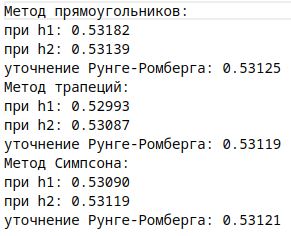
\includegraphics[width=.9\textwidth]{lab3.5}
\caption{Вывод программы в консоли}
\end{figure}

% \vfill

% \begin{figure}[h!]
% \centering
% \includegraphics[width=.9\textwidth]{lab5_taylor}
% \caption{Решение с аппроксимацией граничных условий со вторым порядком}
% \end{figure}
\pagebreak

\subsection{Исходный код}
% \lstinputlisting[language=C++]{matrix.cpp}
% \begin{lstlisting}
\lstinputlisting{include/lab3_5.cpp}
\lstinputlisting{include/integrate.h}
\lstinputlisting{include/interpolation.h}
\lstinputlisting{include/polynom.h}
% \end{lstlisting}
% \lstinputlisting{matrix.cpp}
% {../../include/matrix.cpp}
% \pagebreak
% \lstinputlisting[title=\texttt{parabolic\_pde.hpp}]{../../include/partial_differential/parabolic_pde.hpp}
% \pagebreak
% 